\section{Introduction} 

The ULTRACAM high-speed photometry camera (hereafter, ULTRACAM) had its `first-light' at the 4.2m William Herschel Telescope (WHT) on the 16th of May 2002. Since then it has been used on many occasions at three telescopes, namely the WHT, La Palma, Islas Canarias, the 8.2m Very Large Telescope (VLT), Cerro Paranal, Chile and the 3.5m New Technology Telescope (NTT), La Silla, Chile. During the last 12 years, a substantial ULTRACAM data archive has been created. These data contain far more objects than have been reduced  and studied in the course of scientific research on ULTRACAM so far. If an automated data reduction pipeline was built, it would enable a more complete investigation of the archive, by making available reduced photometry for many thousands of objects. This might lead to interesting discoveries and findings. 

ULTRACAM was specifically designed to perform high-speed photometry of faint objects in three filters. These design attributes are fundamental to understanding the scientific value of ULTRACAM.  High-speed photometry is used to observe astronomical phenomena that occur on short timescales. Observations in astronomy often rely on long exposures to capture enough light in order to perform measurements. The general assumption is that the objects we are looking at do not change on very short timescales (\textless~seconds). This is not true for all objects. Some objects are variable on timescales of much less than 1 second. At the extreme end of this scale are pulsars, which spin at a rate of 100s of times per second \citep{pulsarreview}. Compact objects that are in binary systems that eclipse as seen from the Earth can disappear in less than a minute. Some short period eclipsers have ingress times as short as 30 seconds, making steep eclipse profiles. In fact, a class of these stars, cataclysmic cariables (CVs) with strong magnetic fields, have a very compact bright region that can disappear in less than a few seconds \citep{WarnerBook}. In addition, these systems also display rapid variability due to the interaction of the accretion stream with the other elements in the system. The stream itself is not a contiguous object, but can be formed of discrete 'blobs' of plasma that cause a phenomenon known as 'flickering'. Exoplanet transits may last several hours, but their ingress and egress times can last for tens of minutes or so \citep{exoplanettransits}. Pulsating white dwarfs stars show variations in their light output on timescales of a few minutes \citep{wingetreview}.  High-speed photometry was developed in order to study these objects. 

ULTRACAM is installed on some of the larger telescopes in the world. Using large telescopes assists high-speed photometry as the increased light gathering power of the large mirrors allows for shorter exposure times compared to what would be needed at smaller telescopes. The combination of ULTRACAM with large telescopes like the VLT has enabled researchers to take high-speed ($\Delta t<5~\mbox{seconds}$) photometric measurements of targets such as GU Mus, which is a 20th magnitude (in quiescence) X-ray binary \citep{tariq2010}. It has also been used to take even higher speed measurements of objects such as V834 Cen, a 17th magnitude polar CV at a time resolution of $\sim 0.05$ seconds.

\begin{figure}
\centering
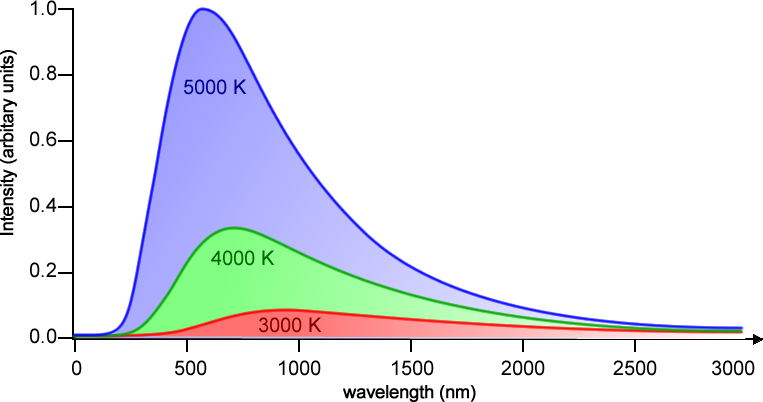
\includegraphics[width=90mm]{images/wienslaw.png}
\caption[Caption for LOF]{The distribution of energy as a function of wavelength for a black body\protect\footnotemark. Stars can be approximated as black bodies, radiating their energy according to this relationship. Hotter stars emit their flux at shorter wavelengths than cooler stars. By measuring an object's flux at various wavelengths, we can deduce information about the temperature of the object.}
\label{fig:wienslaw}
\end{figure}
\footnotetext{Diagram taken from: \url{http://www.spaceflight.esa.int}}
Since stellar objects can be treated (to a first approximation) as black bodies, we use the colour of the object to give us an indication of its temperature. Black bodies radiate at different wavelengths depending on their temperature according to Planck's Law, with the maximum flux at a wavelength predicted by Wien's Law, $\lambda_{max}\mbox{T} = 2.898\times10^{-3}\mbox{mK}$, see Fig. \ref{fig:wienslaw}. By using pre-defined filters we can measure the flux at different wavelengths and thereby derive colour and hence an indication of the object's temperature. If the object is an eclipsing binary, the colour changes during the eclipse allow us to infer the temperature of each component in the system. During an exoplanet transit, subtle changes in colour during primary transit and also comparing the colours during, and just before and after secondary transit, allow researchers to determine the colour of the planet and therefore give an indication of the composition of its surface and/or atmosphere \citep{2012ApJS..201...36B}. For an intrinsic variable, such as a $\delta$ Scuti star, the colour changes during a pulsation cycle allow researchers to monitor the temperature changes on the star's surface during the pulsation cycle \citep{KurtzBook}. By measuring three colours simultaneously, ULTRACAM enables the study of high speed colour and temperature changes. 

\section{Candidate objects}
ULTRACAM is constantly taking images of a region that is several arc minutes in size (as shown in Table \ref{tab:pixelscale}), it will also capture data for any other objects that just happen to be in the field (or `passing-through' the field) during the run. One of the main reasons for automating the reduction pipeline is that it  might allow the serendipitous discovery of objects that, although not the intended targets of the run, are nevertheless displaying some kind of variability. Depending on the size and orientation of the windows that the observer has selected and how crowded the field of view is, many objects could have been recorded that have not had light-curves produced yet. Producing and analysing these new light-curves will hopefully allow the discovery of new variable objects.  In this section we list some of the object classes that might be revealed through a closer inspection of the ULTRACAM data.


\begin{table}
	\caption{The field sizes and pixel scales of ULTRACAM on each of the three telescopes.}
	\begin{tabularx}{\textwidth}{l l l l}
		\hline
		Telescope & Field size        & Pixel scale & Orientation \\
		                  & (arc minutes) &   (arc seconds/pixel) & \\
		\hline
		WHT & 5.1x5.1 & 0.30 & N(up), E(left)\\
		NTT & 6.0x6.0 & 0.35 & N(up), W(left)\\
		VLT & 2.6x2.6 & 0.15 & N(up), W(left)\\
		\hline
	\end{tabularx}
	\label{tab:pixelscale}
\end{table}


\subsection{Eclipsing binaries}
Many of the stars in the galaxy are not isolated, solitary stars, but reside in multiple star systems. It is estimated that the field star population in the solar neighbourhood consists of 50\% binary systems \citep{binaryfraction}. A proportion of these systems will be viewed edge-on from Earth ($i \sim 90^\circ$) and therefore eclipses will occur at least once per orbit. Eclipses are seen as a drop in flux and the eclipse shape and depth indicates the relative sizes and different surface brightness of the two objects in the system. If the two objects differ in temperature, then the eclipse will show a change in colour which can be estimated using the relative fluxes measured in the 3 channels. Since the typical run length for ULTRACAM is about 1-3 hours, we are biased towards detecting binaries with short orbital periods (\textless 1 day). 

\subsection{{W UMa} systems}
{W UMa} systems are binary systems in which both stars have filled their Roche lobes and their atmospheres are effectively merged, although their cores are separate and in orbit about each other \citep{Lucy68}, see Fig. \ref{fig:wumadiagram}. Since they share the same outer layers, or common envelope, this is usually assumed to be at a more or less uniform temperature. The stars are not necessarily of equal mass and their cores will be at different temperatures according to the mass-temperature dependence for main sequence stars. Higher mass stars will have higher core temperatures. The unusual requirements of the thermodynamics of W UMa stars implies that they are limited to certain spectral types as discussed by \citet{Lucy68}.  As these objects rotate, we see a change in flux due to the non-spherical shape of each star as they present different surface areas towards the Earth. Since the stars are in contact with each other, eclipses are visible across a wide range of inclinations ($90^\circ > i > 30^\circ$). The depth of the flux change will depend on the inclination of the orbit, although at a maximum we expect to see a change in flux of about 50\% \citep{Lucy68}. If we are seeing the orbit pole-on, with inclination $i \sim 0$, then we will see very little variability. At inclinations of $i \sim 90$ we will see the maximum drop in flux of approximately $\sim50\%$. Since the temperature of the common envelope surrounding these bodies is expected to be close to uniform there should be only small changes in colour during the orbital cycle. W UMa periods fall in the 6 to 20 hour range and should therefore be obvious in the ULTRACAM data for runs of duration 30 minutes or more. 

\begin{figure}
\centering
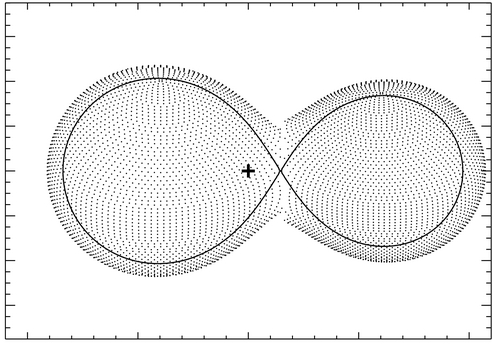
\includegraphics[width=90mm]{images/wuma_diagram.png}
\caption{Diagram showing the layout of a {W UMa} contact binary. The surface of the outer envelope is defined by a Roche equipotential. The $+$ symbol denotes the centre of gravity of the system.  From \citet{0004-637X-764-1-62}. }
\label{fig:wumadiagram}
\end{figure}

\subsection{Ellipsoidal variables}
Stars in binaries that are not in contact but still sufficiently close to each other to cause tidal distortion of one or more of the components will show variability for the same reason as the {W UMa} stars. The projected area of the star presented towards the Earth varies over the orbital cycle. The typical change in brightness of an ellipsoidal variable is about 0.1 magnitudes or a 10\% change in flux. Orbital periods should be similar to those of the {W UMa} category, about 6-20 hours and should be visible in the ULTRACAM data. For a review of the study of this class of stars see \citet{EllipsoidalReview1985}.

\subsection{Cataclysmic variables}
Cataclysmic variables are objects containing two stars in a semi-detached state with one of the stars filling its Roche lobe and streaming material onto the companion. The companion in this case is a white dwarf. The white dwarf has a mass between $0.4 M_{\odot}$ and $1.4 M_{\odot}$, yet a radius that is similar to the Earth. The white dwarf's surface is, therefore, a long way from the gravitational equilibrium point (Lagrangian L1 point) where this flowing material leaves the donor star and starts to fall inwards. Since the material has its own angular momentum, it cannot fall directly towards the white dwarf, but orbits around it, usually forming an accretion disc through which it eventually migrates onto the white dwarf's surface. A sketch of the force potentials for matter in such a system is shown in Fig. \ref{fig:rochepotential}.

\begin{figure}
\centering
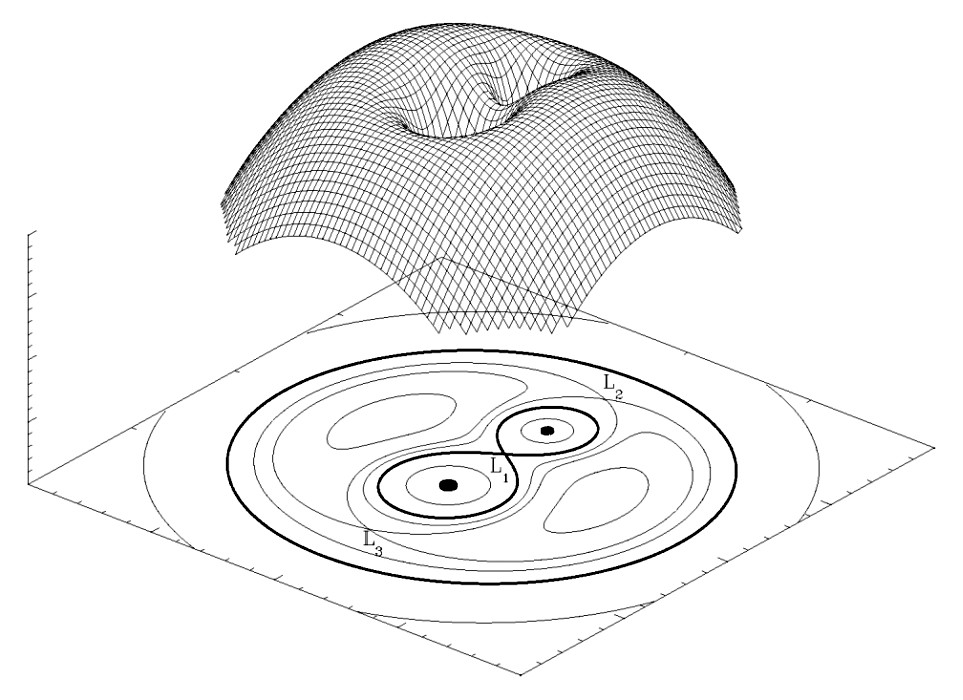
\includegraphics[width=90mm]{images/rochepotential.jpg}
\caption{Schematic plot of the potential field for a test object placed in the area surrounding a two body rotating system, such as a binary star system. The `L' points mark position were a body would feel zero force. The `L\textsubscript{1}' point is where the accretion stream begins in a cataclysmic variable.}
\label{fig:rochepotential}
\end{figure}
\footnotetext{Diagram taken from: \url{http://hemel.waarnemen.com/Informatie/Sterren/images/potential.jpg}}

Cataclysmic variables are highly variable on many different timescales. On the timescale of centuries, they can undergo nova explosions where they explode a shell of hydrogen that has been built up on the White Dwarf surface, increasing their brightness by 8-15 magnitudes \citep{HellierBook}. Over a period of weeks to months, their accretion disks can brighten dramatically in `outbursts', increasing by 3-6 magnitudes. On the timescale that is most relevant to a typical ULTRACAM run, we can expect to see eclipses of the white dwarf, bright-spot and disc (assuming this is an eclipsing system) and flickering caused by the accretion stream flowing onto the bright-spot. 

For a complete overview of the field of study of cataclysmic variables, refer to \citet{WarnerBook}. 

\subsection{Intrinsic variables}

\subsubsection{RR Lyrae stars}
RR Lyrae stars are horizontal branch stars that have evolved away from the main sequence and are in the instability strip. Pulsations in RR Lyraes are driven primarily by helium ionisation zones in their interiors. The mechanism by which opacity drives pulsations is known as the $\kappa$ mechanism, \citep{asteroseismology}. They exhibit periods of several hours to a few days and their light-curves are usually non-sinusoidal (with harmonics) and often have a sawtooth shape. The amplitude of the pulsation variation can be between 0.3 and 1.2 magnitudes (corresponding to a change in flux by a factor of 1.3 to 3.0 times). The colours change significantly during the cycle as the surface temperature rises and falls and this should be evident in the ULTRACAM data. 

\subsubsection{$\delta$ Scuti stars}
$\delta$ Scuti stars are driven by similar mechanisms to the RR Lyraes but are more massive stars and are still on the main sequence. They exhibit non-radial pulsation modes which have shorter characteristic periods and smaller amplitudes. Typical periods for the oscillations in $\delta$ Scuti stars range from 18 minutes to 8 hours, with amplitudes up to $\sim \mbox{0.1 mag}$ \citep{KurtzBook}. Like the RR Lyraes, the surface temperature of the star changes during the pulsation cycle and we would expect to see a colour modulation in the light-curve. 

\subsubsection{Pulsating White Dwarfs}
White dwarf stars pass through a region of the HR diagram that can be viewed as an extension of the instability strip. In this region, the white dwarf will experience a similar driving mechanism to that which drives pulsations for the main sequence and horizontal branch stars, namely the $\kappa$ mechanism. The zone where this mechanism is active is the white dwarf's thin hydrogen or helium atmosphere. Pulsating hydrogen white dwarfs are known as {DAVs} or {ZZ Ceti} stars and helium white dwarfs as {DBV}s. The location of the instability strips for each of these varieties of pulsating white dwarf is shown in Fig. \ref{fig:wdinstability}. Pulsating white dwarfs they have a fairly complex oscillation pattern, with many frequencies, as they oscillate with many modes excited. Nevertheless, a pulsating white dwarf should be fairly obvious when observed with ULTRACAM. The oscillations will have periods of a few minutes and amplitudes on the order of 0.1 mag. Lower amplitude pulsations occur in these object, especially in the higher order modes, but these are not detectable with current instruments.  

\begin{figure}
\centering
\includegraphics[width=90mm]{images/wd_instability_strip.png}
\caption{An HR diagram showing the locations of the three white dwarf instability strips, taken from \citet{wingetreview}. The grey line is a 13-Gyr isochrone with z = 0.019 from \citet{Marigo2008}.}
\label{fig:wdinstability}
\end{figure}
\footnotetext{Diagram taken from: \url{http://hemel.waarnemen.com/Informatie/Sterren/images/potential.jpg}}

Pulsations in white dwarfs stars are reviewed in \citet{wingetreview}.

\subsection{Flare stars}
Flare stars are red dwarf stars that undergo flares in their atmospheres resulting in rapid changes in brightness on timescales of minutes to hours, see Fig. \ref{fig:flare}. Typical flare rates for the flare star {UV Cet} are about every 2.5 to 6 hours. In the optical region, flares are expected to appear as fast rises with an exponential decay lasting minutes to hours. During the flare, the brightness increases by a factor of many times \citep{typicalflares}. Flares have also been shown to exhibit colour changes and there is evidence for an anti-correlated time-evolution between the relative flux and the flare colour. ULTRACAM has been used to measure colour changes during flare events \citep{ULTRACAMFlare}. If flare events are happening to objects in an ULTRACAM run, they should be very obvious in the reduced data light curves.  


\begin{figure}
\centering
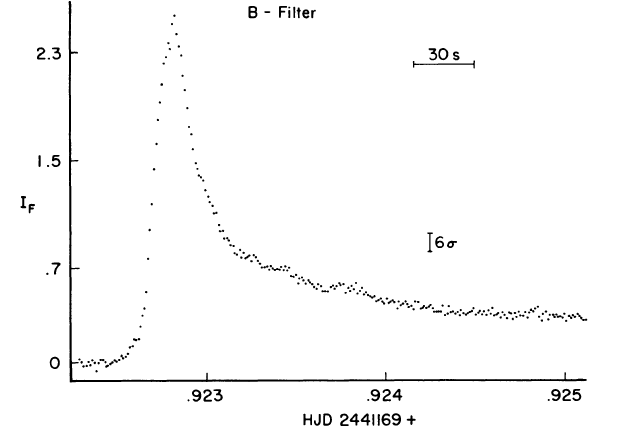
\includegraphics[width=110mm]{images/EQ_Peg_typical_flare.png}
\caption{A light-curve of a typical flare event for EQ Peg, observed in the Johnson B filter. The scale of the y-axis is the intensity in counts as a fractional increase in the intensity from the star's quiescent state minus 1. The diagram is taken from \citet{typicalflares}. }
\label{fig:flare}
\end{figure}

\subsection{Asteroids}
Solar system objects such as asteroids should be visible in the ULTRACAM archive. Main asteroid belt and near-Earth objects are likely to move across the field at a rate of a few arc seconds per minute, meaning that they would cover a fair fraction of the exposed CCD during the course of a 1-2 hour run of the ULTRACAM. We can expect a $\sim 300\,\mbox{m}$ diameter near-Earth object to have an apparent magnitude in V of around 15 \citep{neosmalltelescope} which is bright enough to be clearly visible in most ULTRACAM observations. 

Kuiper belt objects will have apparent magnitudes of around $V\sim 20$ and would move only a few arcseconds per hour. It is fairly unlikely (although not impossible) that one of these objects would be visible in an ULTRACAM run. Kuiper belt objects are, of course, suspected to be within one or two degrees of the ecliptic. 

\section{The ULTRACAM instrument} 
ULTRACAM is an ultrafast, triple-beam, dichroic CCD camera, and has helped open up simultaneous multiband, sub-second time domain astronomy, \citep{dhillon07}. 

\subsection{Camera Optics}

\begin{figure}
\centering
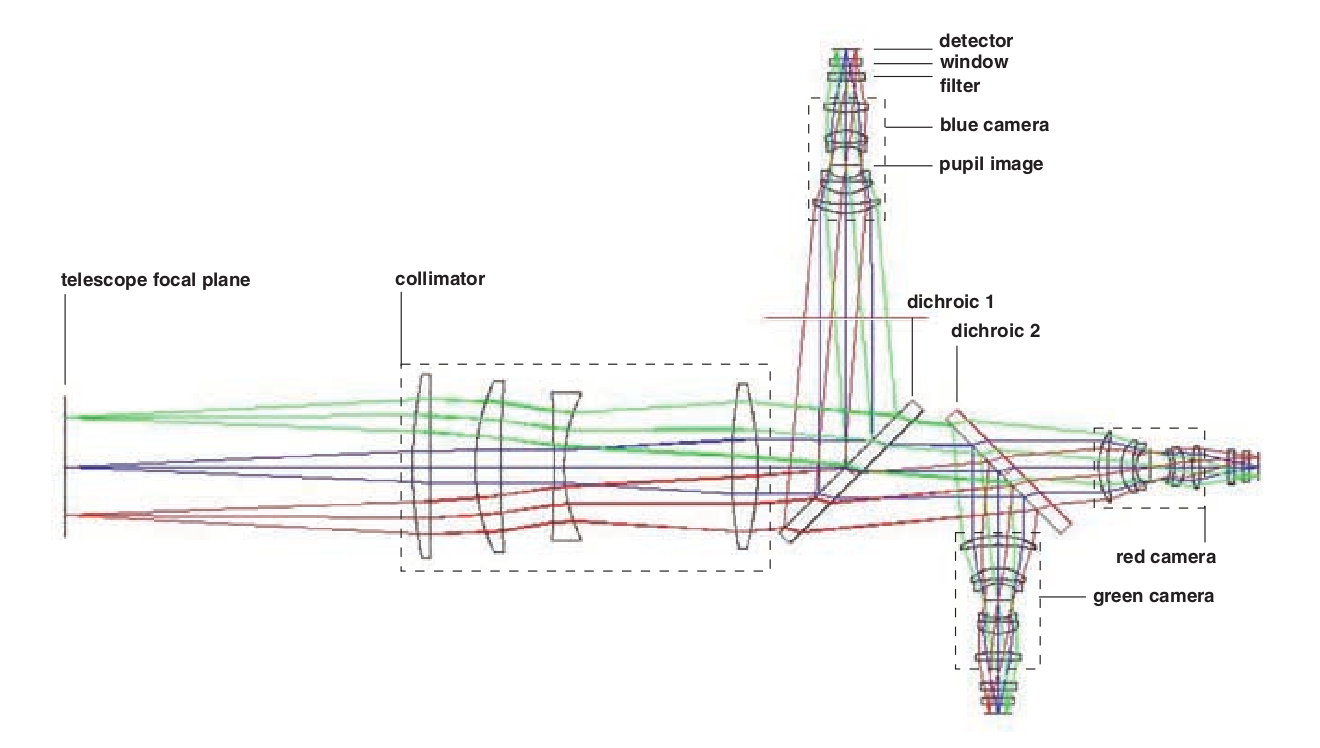
\includegraphics[width=120mm]{images/ucamoptics.png}
\caption{A ray-trace through the ULTRACAM optics, showing the major optical components: the collimator, dichroics, cameras, filters and detector windows. The diagram is to scale – the largest lens is in the collimator and has a diameter of 120 mm. The diagram is taken from \citet{dhillon07}.}
\label{fig:optics}
\end{figure}

The optical layout of ULTRACAM is shown in Fig. \ref{fig:optics}. ULTRACAM has three CCD detectors enabling it to capture data in three colour bands simultaneously. Two dichroic beamsplitters divide the light from the collimator into three beams, which shall hereafter be referred to as the `red', `green' and `blue' channels. The three CCD detectors are mounted at right angles to each other on the camera. Therefore, each detector is at the end of a slightly different optical path. The images produced on each of the three CCDs chips are of the same field of view but with very slightly different orientations, distortions and offsets. Towards the edges of the chips, these differences can be on the order of 10 pixels from channel to channel. 

In general, the exposures are synchronised across all three detectors, meaning that all three CCDs start their exposure, stop their exposure and read-out at the same time. It is, however, possible to have the detector in the blue channel remain exposed and not read-out while the other two are going through multiple exposures and read-outs. This is to allow for longer exposures where there might be less flux in the blue CCD. Reduced flux in the blue CCD is caused by several factors, including lower transmission of the optics and atmosphere for blue light, the reduced sensitivity of the CCD detector to blue light and the low intrinsic flux of most astronomical objects in this region of the spectrum.

\begin{figure}
\centering
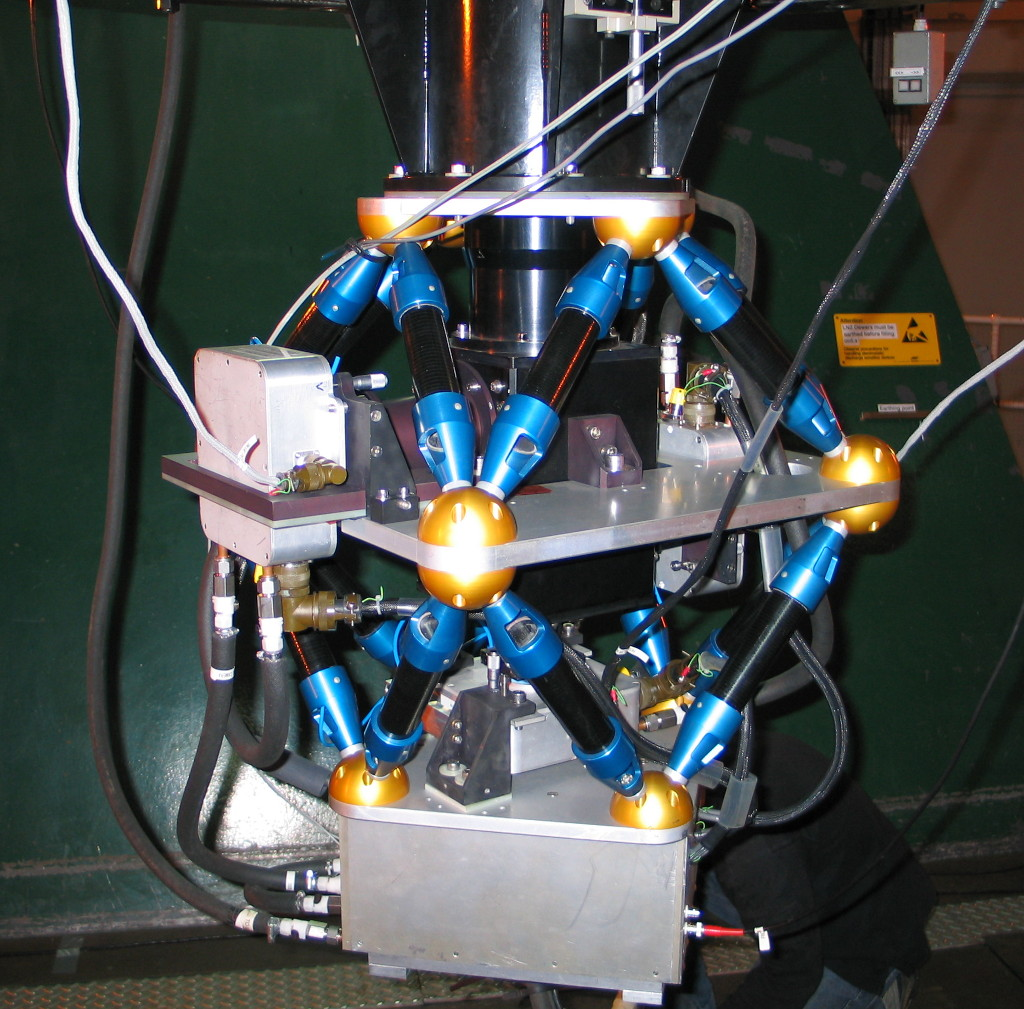
\includegraphics[width=90mm]{images/IMG_0121_scaled.JPG}
\caption{ULTRACAM being commissioned in May 2002.}
\label{fig:ultracam}
\end{figure}

\subsection{Filter sets}
The filters for each channel can be altered by the observer. In usual configurations, the SDSS filters (u, g, r, i, z) are used, but there are a selection of narrow-band filters that can be substituted, depending on the scientific measurements that the observer is performing. Figure \ref{fig:responsecurves} shows the response curves of the ULTRACAM camera combined with the SDSS filter set and the atmosphere. 

\begin{figure}
\centering
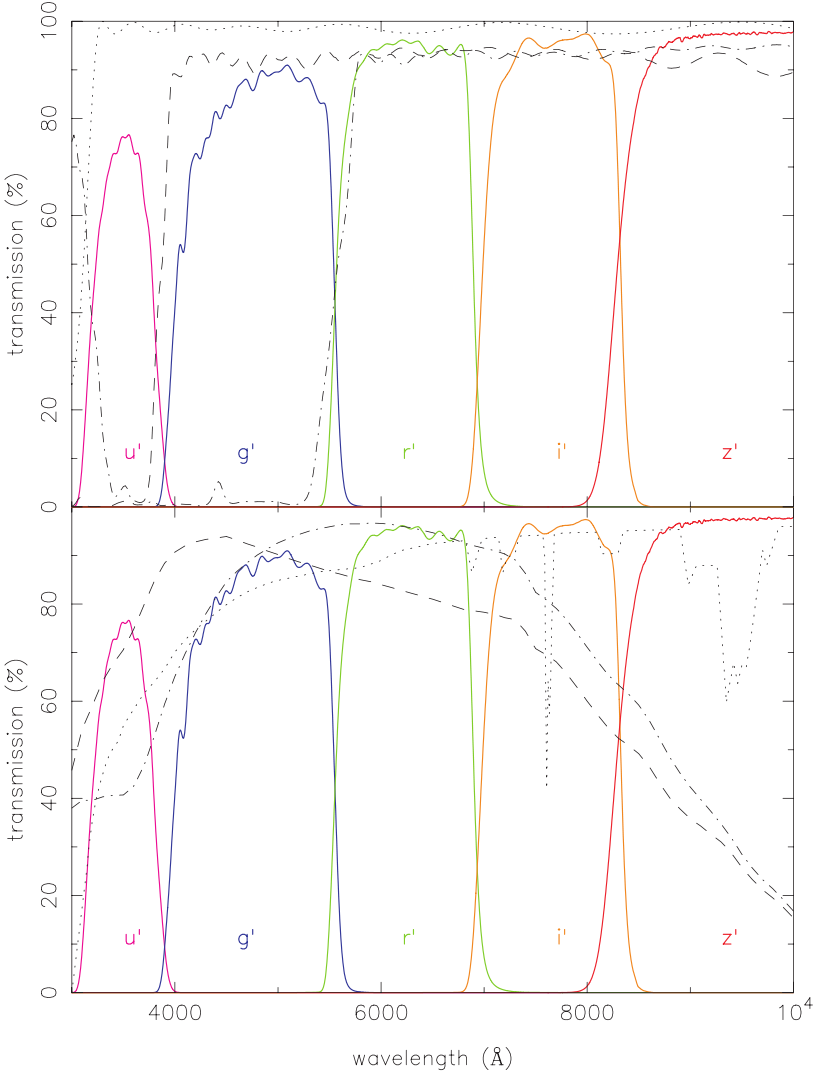
\includegraphics[width=130mm]{images/ucamresponsecurves.png}
\caption{The response curves of ULTRACAM with the SDSS filter set. The upper plot shows the SDSS filter set, the response of the antireflection coating used on the lenses (dotted line) and the two dichroics (dashed line and dash-dotted line). The lower plot shows response of the SDSS filter set and the atmosphere (per unit airmass). The figure is taken from \citet{dhillon07}.}
\label{fig:responsecurves}
\end{figure}


\subsection{Field size and pixel scale}
ULTRACAM is mounted on one of the three telescopes mentioned in the introduction of this chapter (VLT, NTT, WHT). Field sizes, pixel scales and orientations are summarised in table \ref{tab:pixelscale}. The orientations quoted refer to when the camera is not rotated. 

\subsection{High-speed operation}
A key aspect of the design of the camera is its ability to perform at high cadence, or frames per second. It is possible to have the camera read-out at up to 500Hz (frames per channel per second), \citep{dhillon07}. This makes the camera useful for observations of rapid transient variable events with accurate timing. Although the camera is not often used in this very high-speed mode, there are a few observing runs where the camera has been used for measurements with exposure times of approximately 0.005 seconds. Each CCD has a total pixel area of 2057x1024 pixels. Half of these pixels are masked and never exposed to light. They are used as a temporary buffer for reading out the information captured on the CCD. CCD detectors are normally read-out serially, but in order to decrease the time between exposures, the full image can be moved quickly from the imaging area of the CCD to the storage area and this can then be read-out while the imaging area is once again exposed to light. 

\begin{figure}
\centering
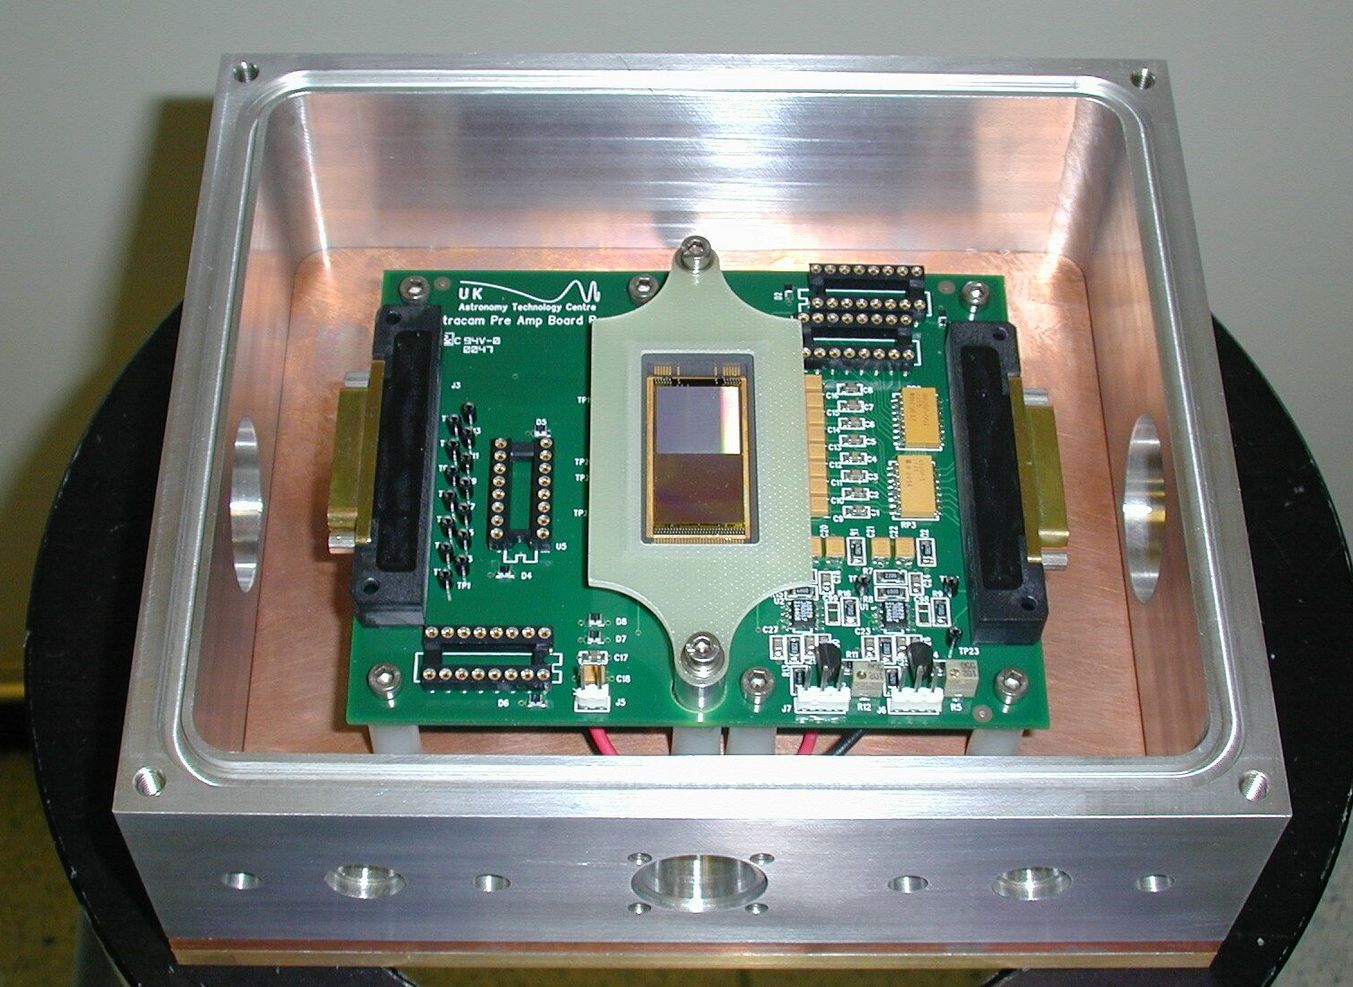
\includegraphics[width=90mm]{images/ccd.png}
\caption{One of the three CCD detectors. The lower half of the chip is masked-off and not exposed to light.}
\label{fig2}
\end{figure}

ULTRACAM gives the observer the option to reduce the area of the detector that is used for the observations. This reduces the chip read-out time and enables the rapid operation of the camera. Reducing the number of pixels recorded also decreases the amount of data storage needed for the run. The observer can define pairs of windows that are centred on the target objects. By making the windows suitably small, the observer can use the camera in extremely high cadence mode. 

The highest cadence mode is called \emph{Drift mode}. This mode uses the storage area of the CCD to store several exposures simultaneously. Only a portion of the imaging area of the CCD is shifted into the storage area. The fact that the camera is not shifting the whole of the imaging area means that it is is ready to be re-exposed sooner than if it was transferring the full-frame. This mode requires that only the lower portion of the imaging area, close to the boundary of the masked and un-masked areas, is used for the exposures. This means that the camera has to be rotated so that the target object (and a suitable comparison star) are positioned correctly. ULTRACAM is therefore designed to be rotated about the optical axis of the telescope in order to allow for this specific object placement. For any particular run, it is possible that we might have any orientation ($0-360^{\circ}$) of the camera relative to the sky coordinates. The ULTRACAM logs do not record this rotation angle. This is an important point to remember when we try to find astrometric solutions for the runs.    

\begin{figure}
  \centering
  \setlength{\fboxsep}{0pt}
  \setlength{\fboxrule}{1pt}
  \fbox{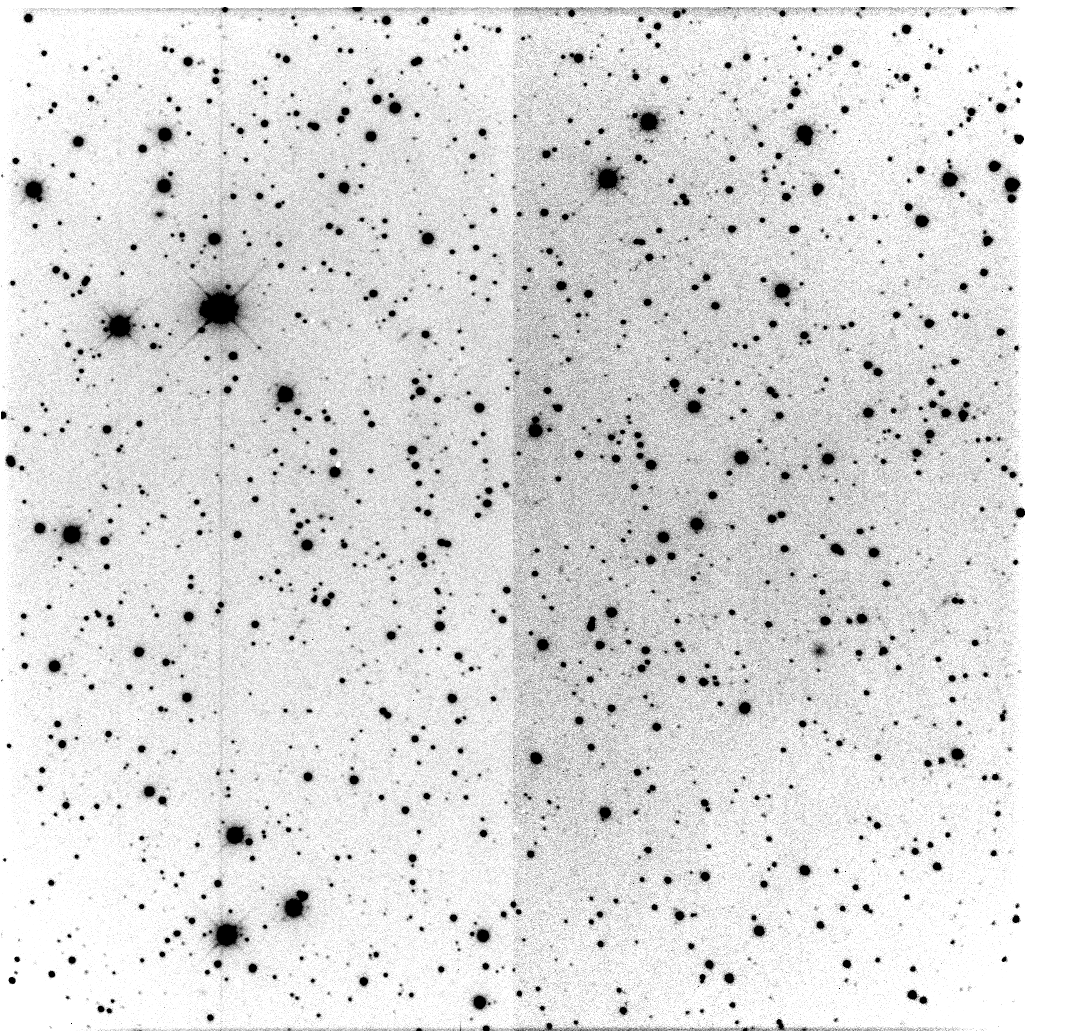
\includegraphics[width=120mm]{images/run010_r_inverted.png}}
  \caption{A fully exposed CCD with 1 pair of windows (512x1024 pixels each).  This mode reads out the full area of the CCD chip. The field of view in this image is approximately 5.1x5.1 arc minutes since it was taken with ULTRACAM mounted on the WHT. The field of view is 6.0x6.0 arc minutes on the NTT and 2.6x2.6 arc minutes on the VLT.}
  \label{fig:KOI-824}
\end{figure}

\begin{figure}  
  \centering
  \setlength{\fboxsep}{0pt}
  \setlength{\fboxrule}{1pt}
  \fbox{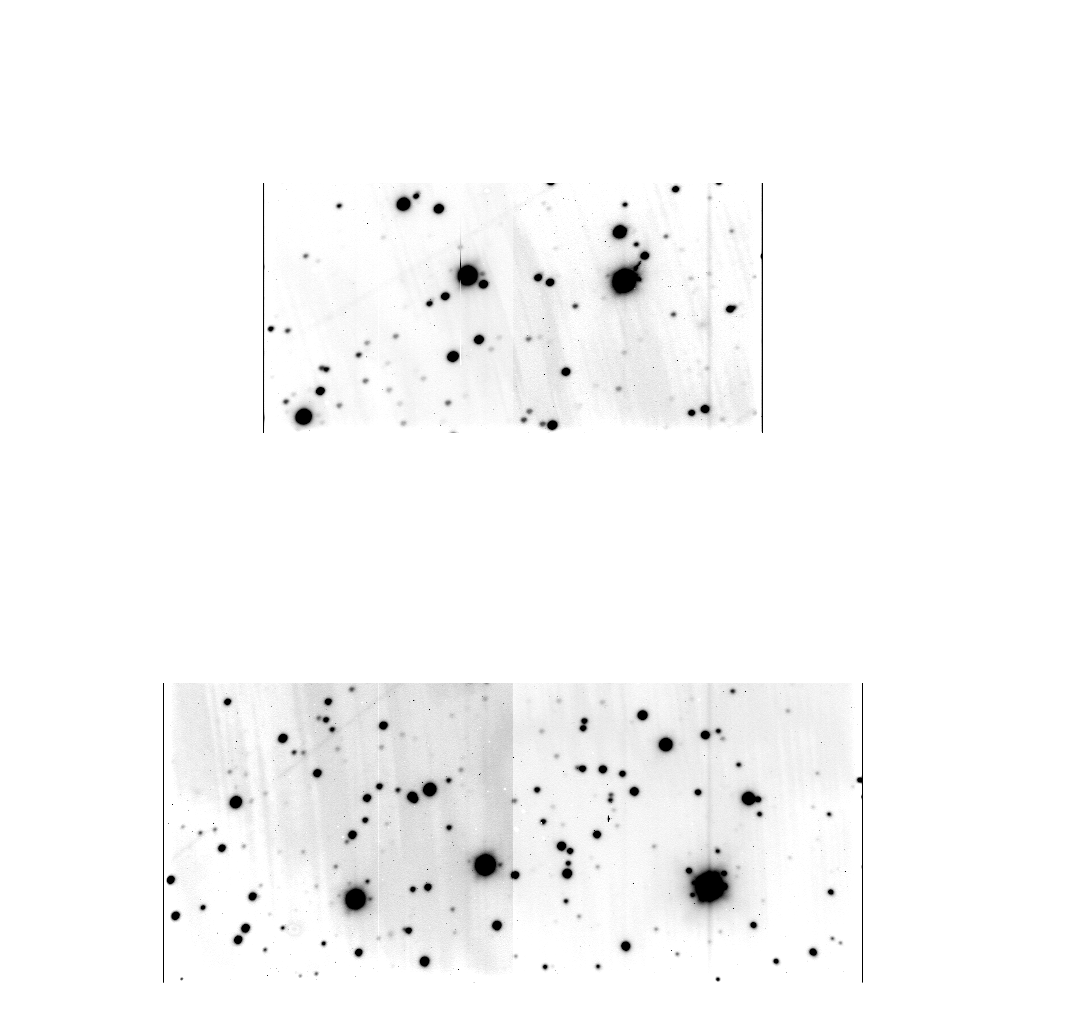
\includegraphics[width=120mm]{images/run016_r_inverted.png}}
  \caption{A masked exposure with 2 pairs of windows (350x300 and 250x250 pixels each, respectively)}
  \label{fig:V713Cep}
\end{figure}

\begin{figure}  
  \centering
  \setlength{\fboxsep}{0pt}
  \setlength{\fboxrule}{1pt}
  \fbox{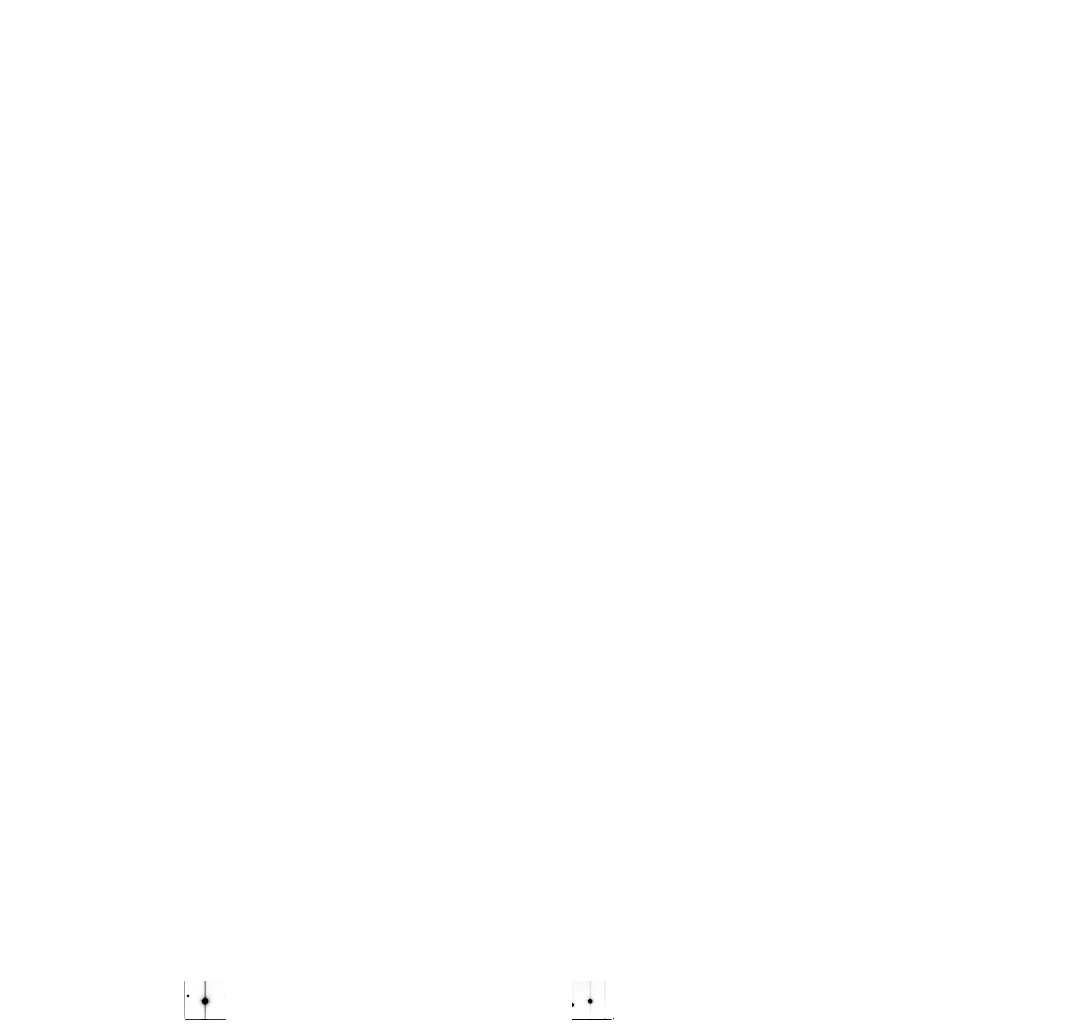
\includegraphics[width=120mm]{images/run018_r_inverted.png}}
  \caption{The camera operating in \emph{drift-mode}. Note the very small windows (172x156 pixels) located at the bottom of the imaging area.}
  \label{fig:V834Cen}
\end{figure}

More details on the camera design and operation can be found in \citet{dhillon07}.

\section{ULTRACAM data}
In nearly all observing runs there is a specific target object defined and the camera and telescope are set up to optimise the observations for this kind of object. Exposure times, filters and field sizes are chosen that are appropriate to the science data that is required. The ULTRACAM archive contains data that consists of measurements taken with a diverse range of these settings. 

\subsection{Data capture}
Typically the camera remains installed on the telescope for a week or so and is used for observations on consecutive nights. Each separate recording of data is called a run. On most nights, many runs are recorded. A run can be defined as a period when the camera is active and gathering data. Not all runs are used for gathering scientific data. Some runs are used for target acquisition and camera calibration. The types of runs are:

\emph{Science runs}: These are the runs that contain the valuable scientific data. They usually comprise the longest portions of the observations during the night, unless the camera is having difficulties or adverse weather conditions are preventing useful astronomical observations.

\emph{Acquisition runs}: These are runs, usually of short duration (ie a few minutes) during which the telescope is being moved in order to place the candidate object(s) in the field of view. The camera may also be rotated in order to align the CCD such that the targets avoid `bad' pixels or are near to the lower boundary of the detector (eg for high-speed readout in drift mode). 

\emph{Flat fields}: At the start and the end of the night (usually during twilight) the observer will take a few runs to create \emph{sky-flats} that will be used later for calibrating the variations in pixel sensitivity across each of the detectors.  Sky-flats are generated by exposing the camera to patches of sky during the twilight. 

\emph{Biases}: Biases are a set of short exposures with the CCD not exposed to light to build calibration readings for measuring the bias of the detector. The bias frame will be subtracted from the observed frames during the reduction process. 

\emph{Timing calibration runs}: One way to check the timing calibration of the camera is to take frames of a well-known, rapidly oscillating source, for example, the Crab Pulsar (PSR B0531+21). The timing of the optical pulses as measured by the camera can then be compared to the expected times for the pulsar. This is used as a standard clock for timing calibration.

\emph{Darks}: Dark frames are taken with the camera exposed to no light, or as close to no light as is physically possible. They are taken over a range of exposure times similar to the exposure times that are used during the science runs and with the detector at a similar temperature. The purpose of the dark frames is to correct for the gradual accumulation of electrons in the pixels of the detector due to thermal noise. The three ULTRACAM sensors are Peltier cooled to $\sim 233\,\mbox{K}$ and at this temperature are expected to deliver a dark current of $\sim0.05\,\mbox{e}^{-}\,\mbox{pixel}^{-1}\,\mbox{s}^{-1}$. This is significantly lower than the expected sky background of $\sim0.3\,\mbox{e}^{-}\,\mbox{pixel}^{-1}\,\mbox{s}^{-1}$ for this camera at a typical site, \citep{dhillon07}. 

\subsection{Typical run length}
Since ULTRACAM is designed for high-speed photometry, observers using the instrument are usually looking for variations that are clearly noticeable on timescales of a few minutes to a few hours. Most science runs last for a few hours at the most. The longest runs are observations of exoplanet transits which can last from about 4 to 7 hours. Sometimes these have a break near the middle of the run if the telescope goes through the meridian. All three of the telescopes on which ULTRACAM is mounted employ `alt-az' mounts, rather than `equatorial' mounts. Alt-az mounts cannot observe directly at the zenith and the run is interrupted for several minutes, while the telescope is repositioned after the zenith `blind-spot'.

Figure \ref{fig:histogram0-600} shows the distribution of run length which shows that a bulk of the runs are shorter than 5 minutes. This is because there are far more acquisition runs, flat-fields and bias runs than there are science runs. There are also many runs that are nominally science runs (and can be used as such) but are short because the observer has noticed something that they would like to change. This could be an adjustment of the focus, binning factor or integration time. The run is then cut short and a new run is started. The longest run length in the 12 year data archive is 566 minutes or 9.5 hours, taken on 25th of April 2010 at the NTT. This was for the observation of a transit of the exoplanet Wasp-15b, \citep{Wasp15b}. The output for this run can be seen at \url{http://deneb.astro.warwick.ac.uk/phrnaw/sitedev/2010-04-25/run020.html}. 

\begin{figure}
  \centering
  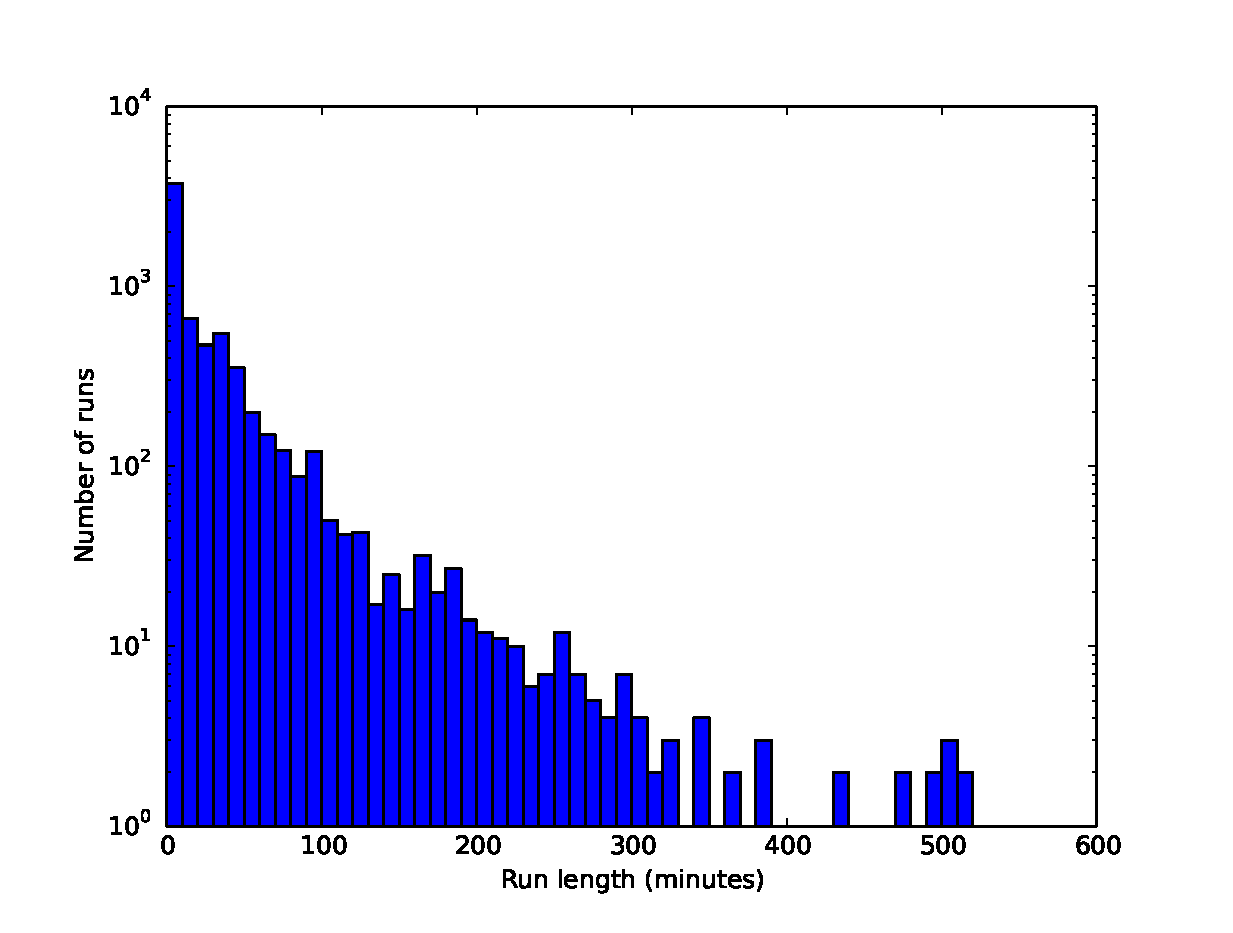
\includegraphics[width=120mm]{images/hist0-600_log.eps}
  \caption{Distribution of run length. Many runs are shorter than 5 minutes, but these are not usually science runs. Note that this is plotted on a logarithmic scale on the vertical axis. }
  \label{fig:histogram0-600}
\end{figure}

\subsection{Run cadences}
Only certain objects, displaying rapid variability, require the highest cadences (\textless 1 second). These are X-ray binaries, polars, pulsars and flare stars. Many other science runs can use the camera with a \textgreater 1 second exposure time. Long runs for exoplanet transit observations often use exposures of 2-3 seconds. The longest exposure times are around 20-25 seconds. This is only required when the object being observed is extremely faint.  

\begin{figure}
  \centering
  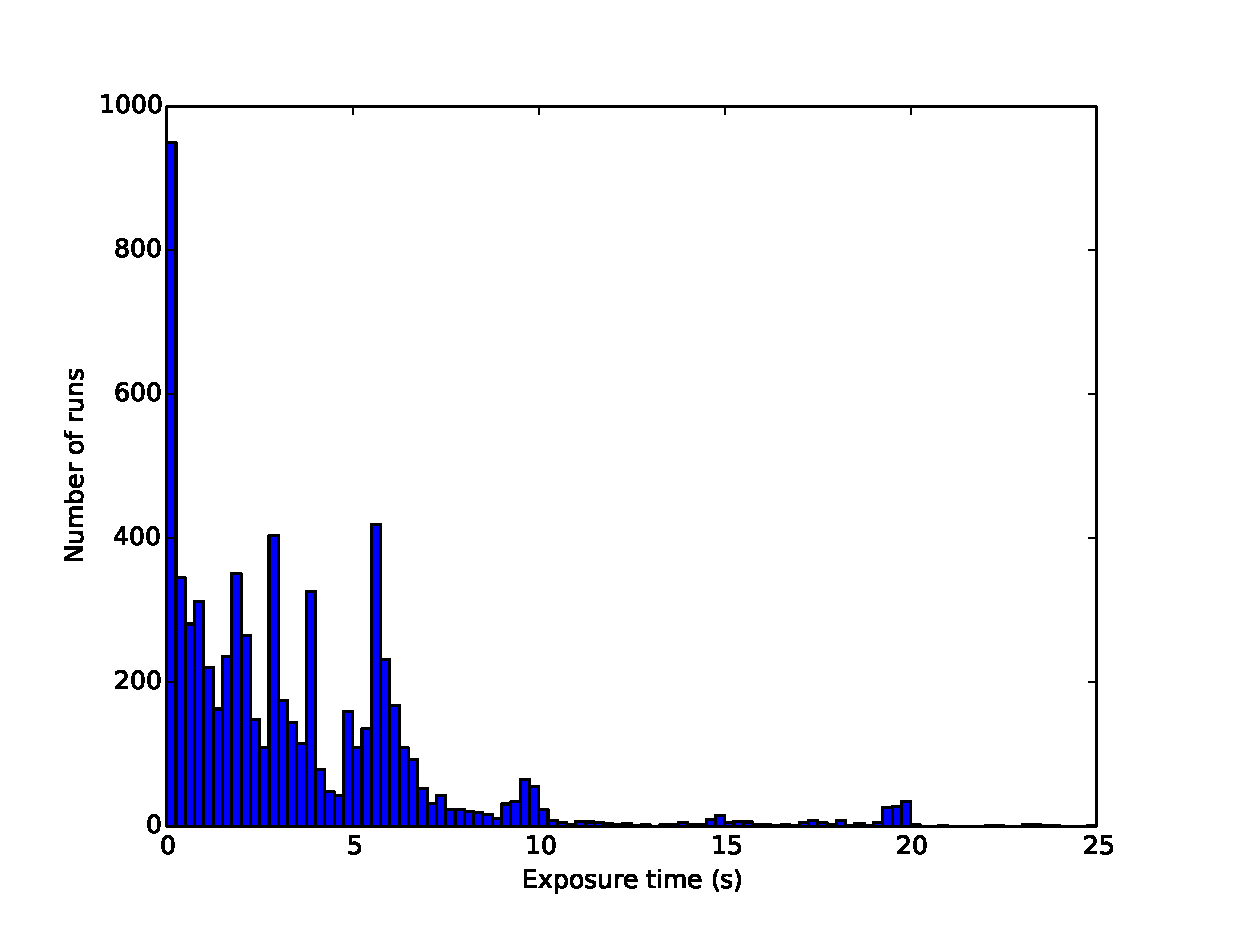
\includegraphics[width=120mm]{images/cadences_hist0-25.eps}
  \caption{Distribution of exposure times used in the science runs.}
  \label{fig:cadences}
\end{figure}

Figure \ref{fig:cadences} shows a distribution of exposure times by run for all of the science runs in the ULTRACAM data archive. There are several groupings apparent in the histogram. Firstly, the very short exposures for the rapidly variable objects, such as polars, pulsars and X-ray binaries. Then there is a cluster of runs with exposure times of 2, 3, 4 and 5.5 seconds. These are typically observations of eclipsing white dwarf binaries. The next cluster occurs at about 10 seconds, which are usually runs for exoplanet transits. The final cluster of run lengths occurs at around 20 seconds and is usually for very faint objects of magnitude \textgreater 19.

\subsection{The data archive}
At the time of writing, the ULTRACAM data archive is \textgreater 10 terabytes. This can be broken down as:
\begin{itemize}
	\item \emph{406} nights on which ULTRACAM was operational at a telescope.
	\item \emph{12,649} runs, including science runs, acquisition runs, flat fields and biases. 
	\item \emph{119,817,742} frames in total. This total includes all the frames for each channel: red, green and blue.
	\item \emph{10.54} terabytes of raw image data.
\end{itemize} 

The data set is relatively large and is housed on a network-mounted storage device that is only available through the internal university computer network. This means that it is not possible to access these data from remote locations (for example, by research collaborators in different institutions). If a researcher needs to results of an observing run, then they need to contact a member of department at the University Warwick or the University of Sheffield (where there is a similar ULTRACAM archive) and request a data reduction. There is no means of accessing or exploring the ULTRACAM data from a remote location. Providing a simple means of accessing these data from remote locations would benefit all of the research collaborators and is one of the aims of this project.

\section{Summary}
There is good motivation for building an automated data reduction pipeline for the ULTRACAM archive. Having a complete set of reduced photometry of all objects in the archive will enable the discovery of new and potentially interesting variable objects of the types described in this chapter. The automated pipeline will also enable greater accessibility of the archive to collaborators. The challenge to building a successful automated pipeline is that it needs to reduce a large amount of raw data that is very diverse in terms of the data size, frame-rates and image size. We describe our solution in the next chapter. 